\documentclass[a4paper,10pt]{article}

\usepackage{graphicx, caption, subcaption}
\usepackage[utf8]{inputenc}
\usepackage[T1]{fontenc}
\usepackage{wrapfig}

\usepackage{hyperref}
\setlength{\parindent}{10pt}
\setlength{\parskip}{1.5mm}
\usepackage{geometry}
\geometry{margin=1.25cm}
\addtolength{\textheight}{-1.5cm}
\setlength{\headheight}{32pt}

\usepackage{amsfonts, amstext, color,
	ifthen, fancybox, multirow, fancyhdr, pgf, tikz,%
	colortbl, array, tabularx
}

\definecolor{bgcode}{rgb}{0.95,0.95,0.95}

\usepackage{url}

\usepackage[french]{babel}
\selectlanguage{french}

%partie concernant la gestion des entêtes
\usepackage{fancyhdr}
\pagestyle{fancy}
\usepackage{lastpage}
\renewcommand\headrulewidth{1pt}
\fancyhead[L]{Interface Homme-Machine Unity}
\fancyhead[R]{Université de Poitiers}
\renewcommand\footrulewidth{1pt}
\fancyfoot[L]{Département d'Informatique}
\fancyfoot[C]{\textbf{\thepage/\pageref{LastPage}}}
\fancyfoot[R]{année 2023-2024}
%fin

\usepackage{enumitem}

\usepackage{listings}

\usepackage{version}
\usepackage{tcolorbox}

\newcounter{Exercice}
\newcommand{\Exercice}[1]{\refstepcounter{Exercice}%
	\ \vspace{0mm} \\ \hspace{0.8cm}%
	\noindent \hspace*{0.5cm} {\bf Question \theExercice :} #1 \vspace{-13mm} \\ %
	\subparagraph*{}%
}

\lstset{language=Caml,basicstyle=\normalsize\tt,keywordstyle=\ttfamily\bfseries\underbar,%
	commentstyle=\normalsize, extendedchars=true, fontadjust=true, columns = flexible, flexiblecolumns=true,
	linewidth=.975\linewidth, backgroundcolor=\color{bgcode}, frame=tlrb, xleftmargin=1cm}

\lstnewenvironment{ocamlcode}
{\lstset{language=Caml,basicstyle=\normalsize\tt,keywordstyle=\ttfamily\bfseries\underbar,%
		commentstyle=\normalsize, extendedchars=true, fontadjust=true, columns = flexible, flexiblecolumns=true,
		linewidth=.975\linewidth, backgroundcolor=\color{bgcode}, frame=tlrb, xleftmargin=1cm,
		literate={à}{{\`a}}1 {è}{{\`e}}1 {é}{{\'e}}1 {ê}{{\^e}}1,
	}}%, framexleftmargin=5mm,frame=box}}
{}

\lstnewenvironment{fsharp}
{\lstset{language=Caml,basicstyle=\normalsize\tt,keywordstyle=\ttfamily\bfseries\underbar,%
		commentstyle=\normalsize, extendedchars=true, fontadjust=true, columns = flexible, flexiblecolumns=true,
		linewidth=.975\linewidth, backgroundcolor=\color{bgcode}, frame=tlrb, xleftmargin=1cm,
		literate={à}{{\`a}}1 {è}{{\`e}}1 {é}{{\'e}}1 {ê}{{\^e}}1 {ç}{{\c c}}1,
}}%, framexleftmargin=5mm,frame=box}}
{}

\lstnewenvironment{javasansbord}
{\lstset{language=Java,basicstyle=\normalsize\tt,keywordstyle=\ttfamily\bfseries\underbar,%
		commentstyle=\normalsize, extendedchars=true, fontadjust=true, columns = flexible, flexiblecolumns=true,
		linewidth=.975\linewidth,frame=,backgroundcolor=,xleftmargin=0cm,
		literate={à}{{\`a}}1 {è}{{\`e}}1 {é}{{\'e}}1 {ê}{{\^e}}1 {ç}{{\c c}}1,
}}%, framexleftmargin=5mm,frame=box}}
{}

\lstnewenvironment{java}
{\lstset{language=Java,basicstyle=\normalsize\tt,keywordstyle=\ttfamily\bfseries\underbar,%
		commentstyle=\normalsize, extendedchars=true, fontadjust=true, columns = flexible, flexiblecolumns=true,
		linewidth=.975\linewidth, backgroundcolor=\color{bgcode}, frame=tlrb, xleftmargin=1cm,
		literate={à}{{\`a}}1 {è}{{\`e}}1 {é}{{\'e}}1 {ê}{{\^e}}1 {ç}{{\c c}}1,
}}%, framexleftmargin=5mm,frame=box}}
{}

\newboolean{versionenseignant}
%%%%%%%%%%%%%%%%%%%%%%%%%%%%%%%%%%%%%%%%%%%%%%%%%%%%%%%%%%%%%%%%%%%%%%%%%%%%%%%%%%%%%%%%%%%%%%%%%%%%%%%%
%__     __            _
%\ \   / /__ _ __ ___(_) ___  _ __
% \ \ / / _ \ '__/ __| |/ _ \| '_ \
%  \ V /  __/ |  \__ \ | (_) | | | |
%   \_/ \___|_|  |___/_|\___/|_| |_|
% _____                _                         _
%| ____|_ __  ___  ___(_) __ _ _ __   __ _ _ __ | |_
%|  _| | '_ \/ __|/ _ \ |/ _` | '_ \ / _` | '_ \| __|
%| |___| | | \__ \  __/ | (_| | | | | (_| | | | | |_
%|_____|_| |_|___/\___|_|\__, |_| |_|\__,_|_| |_|\__|
%                        |___/ 
%% modifiez le booleen ci-dessous pour generer la version enseignant ou etudiant
%% ===> true = version enseignant
%% ===> false = version etudiant
\setboolean{versionenseignant}{true}
%%%%%%%%%%%%%%%%%%%%%%%%%%%%%%%%%%%%%%%%%%%%%%%%%%%%%%%%%%%%%%%%%%%%%%%%%%%%%%%%%%%%%%%%%%%%%%%%%%%%%%%%
% \includeversion{ensnote}
%\excludeversion{ensnote}
\ifthenelse{\boolean{versionenseignant}}{\includeversion{ensnote}}{\excludeversion{ensnote}}

\tcbuselibrary{breakable}


\newenvironment{solution}%
{\begin{tcolorbox}[breakable,colback=red!5!white,colframe=red!75!black,title=Solution]}%
{\end{tcolorbox}}

%\tcblower

\newenvironment{info}%
{\begin{tcolorbox}[breakable,colback=green!5!white,colframe=green!75!black,title=Information]}%
{\end{tcolorbox}}


\newenvironment{attention}%
{\begin{tcolorbox}[breakable,colback=green!25!white,colframe=red!55!black,title=Attention]}%
{\end{tcolorbox}}


\newenvironment{boxcode}%
{\begin{tcolorbox}[breakable,colback=gray!5!white,colframe=black]}%
	{\end{tcolorbox}}
	
	
\begin{document}
	


\title{\vspace*{-1cm}Réalisation d'un système solaire}
\author{\vspace*{-1.5cm}Interface Homme-Machine: Unity
\begin{ensnote}
	(Version enseignant)
\end{ensnote}
}
\date{\vspace*{-1.5cm}version 1}
\maketitle
\thispagestyle{fancy}


Voici les objectifs de ce sujet:
\begin{itemize}
	\item Comprendre l'IDE \texttt{Unity}.
	\item Création d'un projet.
	\item Placer des objets dans l'environnement.
	\item Comprendre la hiérarchie pour différencier transformation locale et globale.
	\item Comprendre le canevas 2D.
	\item Manipuler des widgets classiques.
	\item Exploiter les événements pour ajouter des interactions.
	\item Réaliser des scripts simples pour l'animation.
\end{itemize}


\ifversionenseignant
\begin{solution}
\section{Création du projet}

\begin{enumerate}
	\item Installer  \texttt{UnityHub} et la dernière version de \texttt{Unity}. La version sur laquelle ce tutorial a été réalisée est : \texttt{UnityHub 3.7.0} et \texttt{Unity 2023.3.17f1}.
	\item  Ouvrir \texttt{UnityHub} :
	\begin{itemize}
		\item "\textit{New Project}"
		\item "\textit{3D Core}"
		\item "\textit{Project name}" $\rightarrow$ "\textit{TP1 Solar System}"
		\item "\textit{Location}" $\rightarrow$ choisir le dossier de destination
		\item "\textit{Create Project}"		
	\end{itemize}
\end{enumerate}

	
Une nouvelle scène est générée et l'interface affichée en figure~\ref{fig:new-Unity-scene} s'affiche.
\end{solution}

\begin{figure}[h]
	\begin{subfigure}{\textwidth}
		\begin{center}
			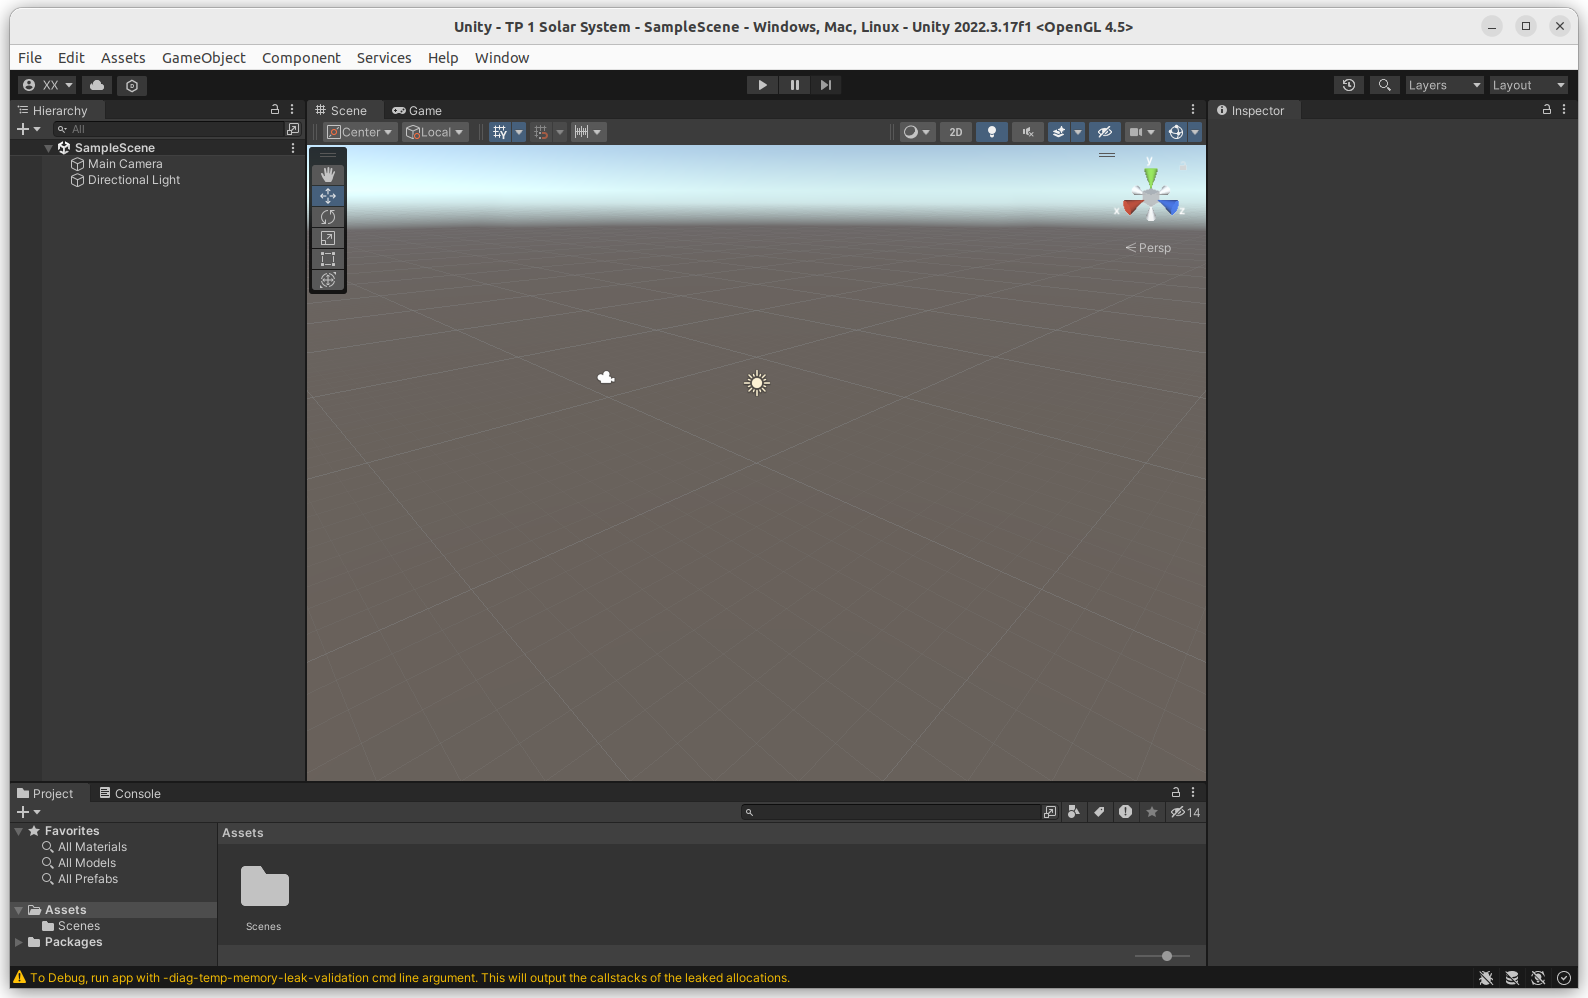
\includegraphics[scale=.30]{fig/new-Unity-scene}
			\caption{Nouvelle scène \texttt{Unity}}
			\label{fig:new-Unity-scene}
		\end{center}
	\end{subfigure}
\end{figure}

\fi 

\ifversionenseignant
\begin{solution}
La fenêtre principale contient deux onglets:
\begin{itemize}
	\item \texttt{Scene} permet de vérifier les propriétés des objets. 
	\item \texttt{Game} affiche la vue de la caméra au démarrage de l'application.	
\end{itemize} 

Attention à bien vérifier que \texttt{Scene} est sélectionné pour mettre en place la scène, sinon on a l'impression que l'interaction est bloquée. Un moyen de s'en assurer est de sauvegarder la scène : si le mode \texttt{Play} ou \texttt{Pause} (voir les icônes en haut de l'interface) a été activé, un message d'erreur apparaît.

Pour arrêter le mode \texttt{Play} ou \texttt{Pause}, il faut cliquer sur les icônes correspondantes pour qu'elles repassent en gris.
\end{solution}
\fi 

%\begin{attention}
%	Le sujet ce fait en deux étapes. Avec une proposition notée de votre interface au bout de 2h (si vous avez fini avant la \textit{deadline} rien ne vous empêche de continuer)!
%	
%	N'oubliez pas d'utiliser les bons réflexes de tout développeur:
%	\begin{itemize}
%		\item Le système de log très bien fait sous Android
%		\item Le mode débogue qui vous permet de voir les valeurs des variables pendant 
%	\end{itemize}
%\end{attention}

\section{Description générale de l'application}

Dans ce TP, nous allons modéliser un système solaire qui n'est pas réaliste physiquement. Pour cela, vous devez réaliser en vous inspirant ce qui a été fait en cours en utilisant la hiérarchie, un système solaire composé des éléments suivants:
\begin{itemize}
	\item \textit{Soleil} qui est au centre de notre animation.
	\item Deux planètes (disons \textit{Terre} et \textit{Mars}) qui tournent autour du \textit{Soleil}.
	\item Des lunes pour chaque planète. Pour information, la \textit{Terre} possède une \textit{Lune} et \textit{Mars} possède 2 lunes (nommées \textit{Phobos} et \textit{Deimos}). 
\end{itemize}


\begin{center}
	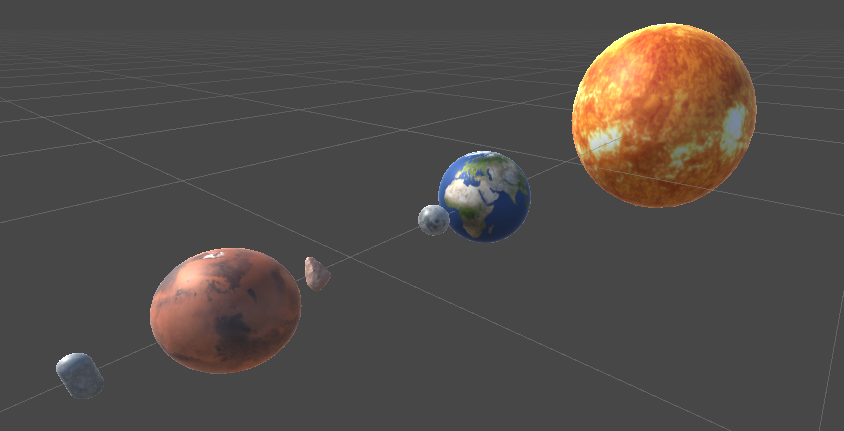
\includegraphics[width=0.7\linewidth]{rc/solarsystem_ez}
\end{center}

L'objectif ici est de réalisez des manipulations d'Unity, vous pouvez/devez expérimenter les points suivants:
\begin{enumerate}
	\item Utilisez la forme primitive Capsule pour Deimos.
	\item Utilisez un maillage produit avec vos mains sous Blender ou \textit{via} un objet quelconque (format \texttt{.obj} de préférence) trouvé sur l'Internet pour remplacer Phobos.
	\item Mettez une texture sur les objets (pas forcément celle des planètes, mais ce que vous voulez).
	\item Modifiez la "\texttt{skybox}" de votre caméra (plusieurs possibilités sont permises, mais utilisez bien la documentation et vos intuitions pour le faire, sans chercher en premier lieu une solution sur le net).
	\item Placez les objets \textit{de manière hiérarchique} pour répercuter les transformations de leur parent.
\end{enumerate}

Vous pouvez utiliser les ressources mises à disposition sur \texttt{UPdago}. Depuis l'interface de \texttt{Unity}~: repérer l'onglet \texttt{Project} et le dossier \texttt{Assets}, dans lequel vous glissez-déposez le dossier \texttt{Images}.

\ifversionenseignant
\begin{solution}
Le contenu du dossier \texttt{Images} et du sous-dossier \texttt{Materials} devrait apparaître sous forme d'icônes. 

Il est possible que l'image \texttt{rosetta}, associée au fichier \texttt{Phobos\_1\_1000.glb} ne soit pas reconnue correctement : cela est dû à un format non supporté en natif par \texttt{Unity}. Deux solutions :
\begin{itemize}
	\item chercher sur un site libre un objets 3D au format \texttt{OBJ}, par exemple sur le site \href{https://turbosquid.com/}{TurboSquid}\footnote{Nécessite une inscription gratuite} (mot-clé: "\textit{rock}" avec filtre "\textit{price = free}"). Une fois l'archive téléchargée, il faut l'ouvrir puis glisser-déposer le dossier correspondant dans \texttt{Assets > Images};
	\item installer un plugin spécifique pour reconnaître le format \texttt{GLTF}:
	\begin{itemize}
		\item Dans l'interface, ouvrir \texttt{Window > Package Manager}.
		\item Cliquer sur le bouton "\texttt{{\large +}} en haut à gauche de la nouvelle fenêtre et sélectionner "\texttt{Add package from git URL...}".
		\item Entrer un lien d'un outil d'import, par exemple \texttt{https://github.com/atteneder/glTFast.git} (Fig.~\ref{fig:glTFast-package}).
		\item \texttt{Unity} importe le \textit{package} et relit automatiquement les \texttt{assets} $\rightarrow$ \texttt{Phobos\_1\_1000.glb} est maintenant reconnue et on peut l'insérer directement dans la scène.
		
	\end{itemize}
\end{itemize}
		
Noter que tous les assets sont automatiquement compilés et le résultat porte l'extension \texttt{.meta}.
\end{solution}


\begin{figure}[h]
	\begin{subfigure}{\textwidth}
		\begin{center}
			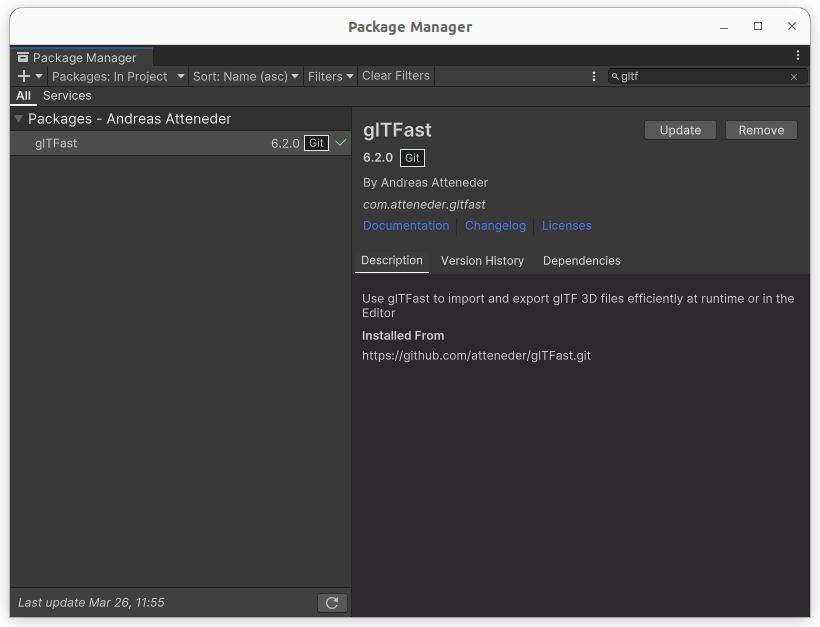
\includegraphics[scale=.50]{fig/glTFast-package}
			\caption{Import du package \texttt{GlTFast}}
			\label{fig:glTFast-package}
		\end{center}
	\end{subfigure}
\end{figure}

\fi 

\ifversionenseignant
\begin{solution}
\subsection{Construction du système solaire}

L'onglet \texttt{Hierarchy} contient les objets définis par défaut avec la nouvelle scène : une caméra \texttt{Main Camera} et une source de lumière \texttt{Directional Light}.

\subsubsection{Directional Light}

Supprimer cette \texttt{Directional Light}. Ce sera le soleil qui fera office de source de lumière.

\subsubsection{Main Camera}

Modifier ses propriétés dans l'onglet \texttt{Inspector} pour correspondre à l'image de la fig.~\ref{fig:main_camera_inspector-01}.
\end{solution}
\begin{figure}[h]
	\begin{subfigure}{\textwidth}
		\begin{center}
			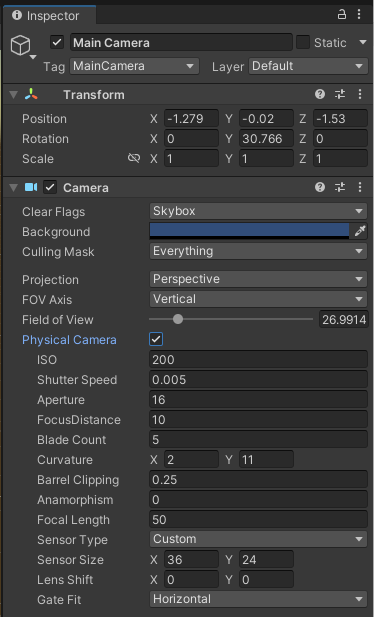
\includegraphics[scale=.50]{fig/main_camera_inspector-01}
			\caption{Propriétés de la \texttt{Main Camera}}
			\label{fig:main_camera_inspector-01}
		\end{center}
	\end{subfigure}
\end{figure}


\begin{solution}
Cliquer sur le bouton \text{Add Component} en bas de l'\texttt{Inspector}. Dans la barre de recherche, entrer \texttt{Skybox}.

On crée ensuite un \texttt{Material} personnalisé:
\begin{itemize}
	\item Dans l'onglet \texttt{Project}, bouton droit de la souris sur \texttt{Assets > Images > Materials} et sélectionner \texttt{Create > Material }.
	\item Donner un nom (par exemple "\textit{8k\_milky-way-2}" au \texttt{Material} qui apparaît (l'extension "\texttt{.mat}" est automatiquement ajoutée).
	\item Dans l'\texttt{Inspector}, les propriétés par défaut du nouveau \texttt{Material} sont affichées.
	\item Cliquer sur le petit cercle à côté de \texttt{Albedo} pour ouvrir le choix de textures. Dans la liste qui s'affiche, sélectionner "\textit{8k\_milky-way-2.jpg}" (ce fichier doit exister au préalable).
	\item L'affichage de la sphère de test en bas de l'\texttt{Inspector} passe du blanc par défaut à la texture sélectionnée.
	\item Sélectionner de nouveau \texttt{Main Camera} dans l'onglet \texttt{Hierarchy}.
	\item Dans le composant \texttt{Skybox}: cliquer sur le cercle à droite du champ \texttt{Custom Skybox} et sélectionner "\textit{8k\_milky-way-2}".  
	
\end{itemize}
\end{solution}
\fi 

\ifversionenseignant
\begin{solution}
	\subsection{Soleil}
	
	\begin{itemize}
		\item Dans l'onglet \texttt{Hierarchy}:  bouton droit > "\texttt{3D Object > Sphere}"
		\item Renommer en "\textit{Soleil}"
		\item Dans \texttt{Inspector}:
		\begin{itemize}
			\item \texttt{Add Component > Light}
			\item Modifier les propriétés de \texttt{Light}
			\begin{itemize}
				\item \texttt{Range}: $30$
				\item \texttt{Mode} : \texttt{Mixed} (voir \href{https://docs.unity3d.com/Manual/LightMode-Mixed.html}{la doc.})
				\item \texttt{Intensity}: $2.6$
				\item \texttt{Shadow type}: \texttt{Soft shadows}
			\end{itemize}
		\end{itemize}
		\item Dans \texttt{Project}, ouvrir le dossier \texttt{Images > Materials}
		\item Vérifier que l'asset "\texttt{2k\_sun}" est présent. Si son aspect est blanc (défaut), lui associer dans l'\texttt{Inspector}:
		\begin{itemize}
			\item \texttt{Albedo}: la texture \texttt{2k\_sun}
			\item \texttt{Emission > Color}: la même texture
		\end{itemize}
		\item Cliquer sur cet asset et glisser-déposer sur le \textit{Soleil} dans la scène ou l'\texttt{Inspector} : le composant \texttt{Material} se met à jour. Laisser les propriétés par défaut.
	\end{itemize}

Le résultat devrait ressembler à celui affiché en fig.~\ref{fig:config-soleil} (en sélectionnant l'onglet \texttt{Game}).
\end{solution}

\begin{figure}[h]
	\begin{subfigure}{\textwidth}
		\begin{center}
			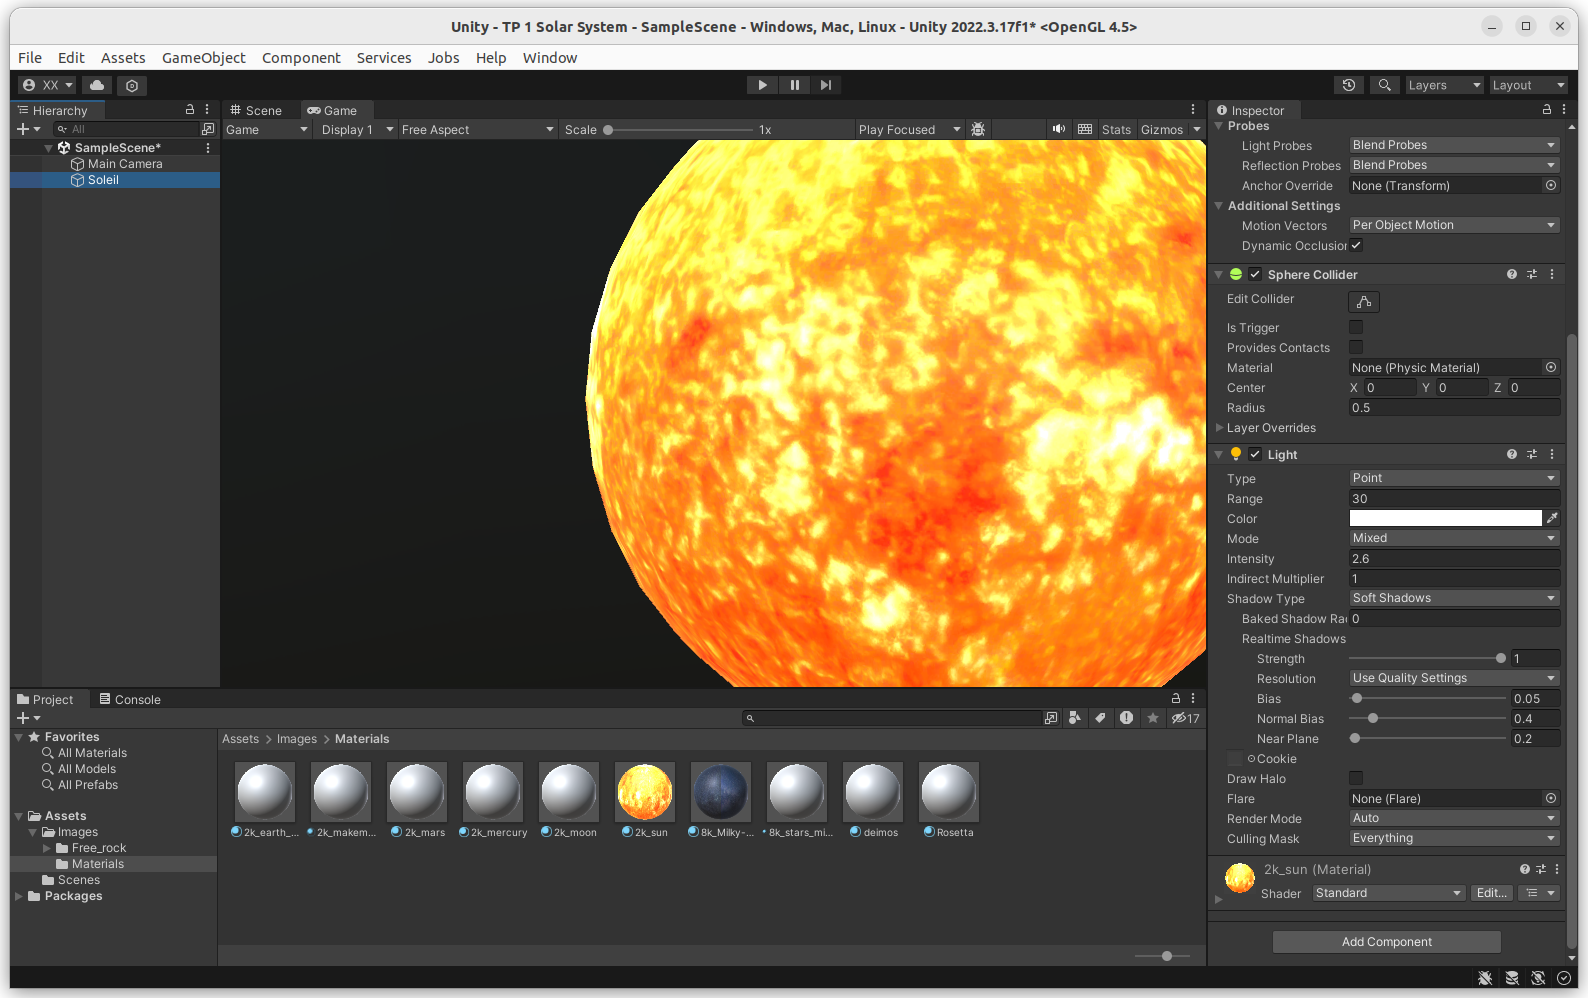
\includegraphics[scale=.30]{fig/config-soleil}
			\caption{Soleil éclairant la scène}
			\label{fig:config-soleil}
		\end{center}
	\end{subfigure}
\end{figure}
\fi 

\ifversionenseignant
\begin{solution}
\subsubsection{Terre}
Ajouter un objet 3D \texttt{Sphere} dans la \texttt{Hierarchy} comme enfant de \textit{Soleil} et le nommer \textit{Terre}.
\begin{itemize}
	\item \texttt{Ìnspector -> Transform}
	\begin{itemize}
		\item \texttt{Position : X = 1.5 ; Y = 0 ; Z = 0} 
		\item \texttt{Scale : X = 0.3 ; Y = 0.3 ; Z = 0.3} (le redimensionnement est calculé \textbf{dans le repère local de l'objet parent} (ici, \textit{Soleil})		
	\end{itemize}
\item Suivre les étapes précédentes utilisées pour affecter une texture au \textit{Soleil} pour affecter une texture à partir de l'image \textit{2k\_earth\_daymap.jpg}.
\item Affecter ce \texttt{Material} directement à \textit{Terre} en le déplaçant depuis \texttt{Project}sur la vue centrale
\item \texttt{Ìnspector -> Shader}
\item \texttt{Advanced Options} : activer \texttt{Enable GPU instancing} et \texttt{Double Sided Global Illumination}
\item Au besoin, déplacer \textit{Main Camera} pour englober le \textit{Soleil} et la \textit{Terre} dans la pyramide de vision.
\end{itemize}

\subsubsection{Lune}
\begin{itemize}
	\item Ajouter un objet 3D \texttt{Sphere} dans la hiérarchie comme enfant de \textit{Terre} et le nommer \textit{Lune}.
	\item \texttt{Ìnspector -> Transform}
	\begin{itemize}
		\item \texttt{Position : X = 0.747 ; Y = 0 ; Z = 0  }
		\item  \texttt{Scale : X = .3 ; Y = .3 ; Z = .3}
	\end{itemize}
	\item Reprendre la procédure d'ajout de texture à partir de l'image \textit{2k\_moon.jpg}. Si ce \texttt{Material} existe déjà, on peut le sélectionner directement en cliquant sur le petit rond dans \texttt{Ìnspector > Mesh Renderer > Materials}.
	\item Ajouter une \texttt{Camera} comme enfant de \textit{Lune} et laisser les propriétés par défaut, puis ajouter une \texttt{Skybox} en reprenant la procédure utilisée pour la \textit{Main Camera}.
\end{itemize}
	\textbf{ATTENTION} : cette seconde caméra est activée par défaut et prend la place de la première dans le \texttt{Game View}. Désactiver cette caméra en désactivant la propriété \texttt{Inspector -> Camera}.

\subsubsection{Mars}
\begin{itemize}
	\item  Ajouter un objet 3D \texttt{Sphere} dans \texttt{Hierarchy} comme enfant de \textit{Soleil} et le nommer \textit{Mars}.
	\item \texttt{Ìnspector -> Transform}
	\begin{itemize}
		\item \texttt{Position : X = 2.27 ; Y = 0 ; Z = 0 }
		\item \texttt{Scale : X = 0.25 ; Y = 0.25 ; Z = 0.25} 
	\end{itemize}
	
	\item Reprendre la procédure d'ajout de texture à partir de l'image \textit{2k\_mars.jpg}.
\end{itemize}

\subsubsection{Phobos}
On a décrit précédemment comment faire interpréter par \texttt{Unity} le fichier relatif à \textit{Phobos}, au format \textit{glTF}. D'autres fichiers sont disponibles sur le \href{https://solarsystem.nasa.gov/resources/2358/phobos-3d-model/}{site de la NASA} par exemple.

\begin{itemize}
	\item  Vérifier que l'objet importé (en fait, une archive) est bien placé dans \texttt{Assets > Images} et l'intégrer dans  \texttt{Hierarchy} comme enfant de \textit{Mars}.
	\item \texttt{Ìnspector -> Transform}
	\begin{itemize}
		\item \texttt{Position : X = -.7 ; Y = 0 ; Z = 0 }
		\item \texttt{Scale : X = 0.01 ; Y = 0.01 ; Z = 0.01} 
	\end{itemize}	
\end{itemize}


\subsubsection{Deimos}
Reprenre la procédure précédente pour intégrer \textit{Deimos} comme lune de \textit{Mars}. On peut utiliser le fichier \href{https://science.nasa.gov/resource/deimos-3d-model/}{sur ce site}.

On a décrit précédemment comment faire interpréter par \texttt{Unity} le fichier relatif à \textit{Phobos}, au format \textit{glTF}. D'autres fichiers sont disponibles sur le \href{https://solarsystem.nasa.gov/resources/2358/phobos-3d-model/}{site de la NASA} par exemple.

\begin{itemize}
	\item  Vérifier que l'objet importé (en fait, une archive) est bien placé dans \texttt{Assets > Images} et l'intégrer dans  \texttt{Hierarchy} comme enfant de \textit{Mars}.
	\item \texttt{Ìnspector -> Transform}
	\begin{itemize}
		\item \texttt{Position : X = 0 ; Y = 1 ; Z = 0 }
		\item \texttt{Scale : X = 0.01 ; Y = 0.01 ; Z = 0.01} 
	\end{itemize}	
\end{itemize}

\end{solution}
\fi 

\section{Premier script pour animer tout cela}

Je vous propose de réaliser le fameux script \lstinline|JeTourne.cs| du cours, qui se contente d'appeler la rotation autour du soleil. Chercher dans la documentation \texttt{Unity}, le rôle de la fonction \lstinline|FixedUpdate()|. Modifiez votre programme pour l'utiliser en conséquence comme dans le cours. Nous ferons en particulier les variables suivantes sans les lier à des boutons ou autre widget:
\begin{itemize}
	\item Ajoutez dans votre script une variable booléenne qui détermine si l'objet en question tourne ou non.
	\item Placez la vitesse de rotation de votre objet  paramètre.
	\item Surchargez les fonctions intéressantes du cycle de vie de votre objet pour en faire un affichage dans la console. 
\end{itemize}

\ifversionenseignant
\begin{solution}
	On place d'abord le script dans le dossier \texttt{Assets}\footnote{On peut créer un dossier \texttt{Scripts} spécifique, au besoin.}. Puis on ajoute ce script à \textit{Soleil} avec un glisser-déposer ou l'\texttt{Inspector}: \texttt{Add Components > Scripts > Je Tourne}. \\
	
Contenu de \lstinline|JeTourne.cs|:

\begin{lstlisting}
using System.Collections;
using System.Collections.Generic;
using UnityEngine;

public class JeTourne : MonoBehaviour
{
	// Par introspection, l'attribut public [mustTurn] est ajoute 
	// sous forme de [Toggle] dans les proprietes du script de l'Inspector, 
	sous le nom [Must Turn]
	// Modifier cette valeur dans l'Inspector modifie cet attribut dans ce code
	public bool mustTurn = true;
	
	// L'attribut [rotationSpeed] est egalement ajoute dans les proprietes du script,
	// sous le nom [Rotation Speed]
	// Modifier cette valeur dans l'Inspector modifie cet attribut dans ce code
	public double rotationSpeed = 5.0;
		
	
	// Start is called before the first frame update
	void Start()
	{
		Debug.Log("Start() de " + gameObject.name);
		mustTurn = true;
	}
	
	// Update is called once per frame
	void Update()
	{
		Debug.Log("Update() de " + gameObject.name);
	}
	
	// FixedUpdate is called at fixed frames. To use with rigid Bodies
	// https://docs.unity3d.com/ScriptReference/MonoBehaviour.FixedUpdate.html
	void FixedUpdate()
	{
		Debug.Log("FixedUpdate() de " + gameObject.name);
		if (mustTurn)
		{
		    Debug.Log("Rotation de " + gameObject.name);
			// Rotation autour de l'axe Y
			//    transform.Rotate(0, 5 * Time.fixedDeltaTime, 0);
			transform.Rotate(0, ((float)rotationSpeed) * Time.fixedDeltaTime, 0);
		}
	}
	
	public void toggle()
	{
		Debug.Log("toggle() de " + gameObject.name);
		mustTurn = !mustTurn;
	}
}
	
\end{lstlisting}

Les logs sont affichés dans l'onglet \texttt{Console}, à côté de \texttt{Project}. On constate que tous les éléments enfants de \textit{Soleil} subissent le même mouvement, avec le \textit{Soleil} comme centre de rotation.
\end{solution}
\fi 

\section{Interaction pour le contrôle du système solaire}

Réalisez l'interface proposée ci-dessous pour le soleil:
\begin{center}
	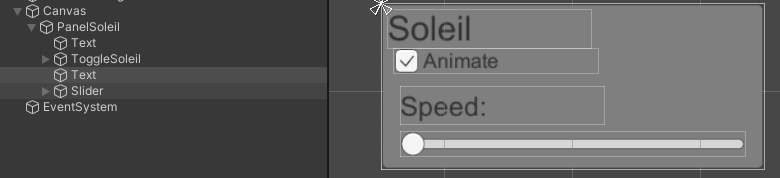
\includegraphics[width=0.7\linewidth]{rc/ui_control_sun_planet}
\end{center}

\ifversionenseignant
\begin{solution}
\subsection{Création du \texttt{canvas}}
\begin{itemize}
	\item Dans \texttt{Hierarchy} : bouton droit : \texttt{UI -> Canvas}. Un objet \texttt{EventSystem} est également automatiquement ajouté.
	\item Parmi les propriétés de ce \textit{Canvas}, les valeurs de position et de dimensions sont automatiquement définies et non modifiables. Ces valeurs seront adaptées au contenu de cet objet.
	\item \texttt{Inspector -> Rect Transform}	(ces valeurs peuvent être différentes selon la configuration de la scène)
	\begin{itemize}
		\item 	\texttt{Pos X = 459 ; Pos Y = 257 ; Pos Z = 0}
		\item \texttt{Width = 918 ; Height = 514   }		
	\end{itemize}	
\end{itemize}

\subsection{\texttt{PanelSoleil}}
\begin{itemize}
	\item Ajouter un \texttt{UI -> Panel} nommé \textit{PanelSoleil} comme enfant de \textit{Canvas}. 
	\item \texttt{Inspector -> Rect Transform}
	\begin{itemize}
		\item  cliquer sur l'icone de positionnement en haut à gauche, \texttt{Stretch / Stretch} et sélectionner \texttt{top / left}
	 \item \texttt{Pivot X = 0 ; Y = 1}. Ces valeurs représentent le point à partir duquel les coordonnées suivantes sont calculées
	\item \texttt{Pos X = 10 ; Pos Y = -40 ; Pos Z = 0}
	\item \texttt{Width = 300 ; Height = 130 }
	\end{itemize}	
	On peut modifier ces valeurs, du moment que ce \texttt{Panel} se retrouve bien à l'intérieur de \textit{Canvas}.	Le panel apparaît sous la forme d'un rectangle gris dans la fig.~\ref{fig:panelSoleil-1} en vue \texttt{Game}.
\end{itemize}
\end{solution}


\begin{figure}[h]
%	\begin{subfigure}{\textwidth}
		\begin{center}
			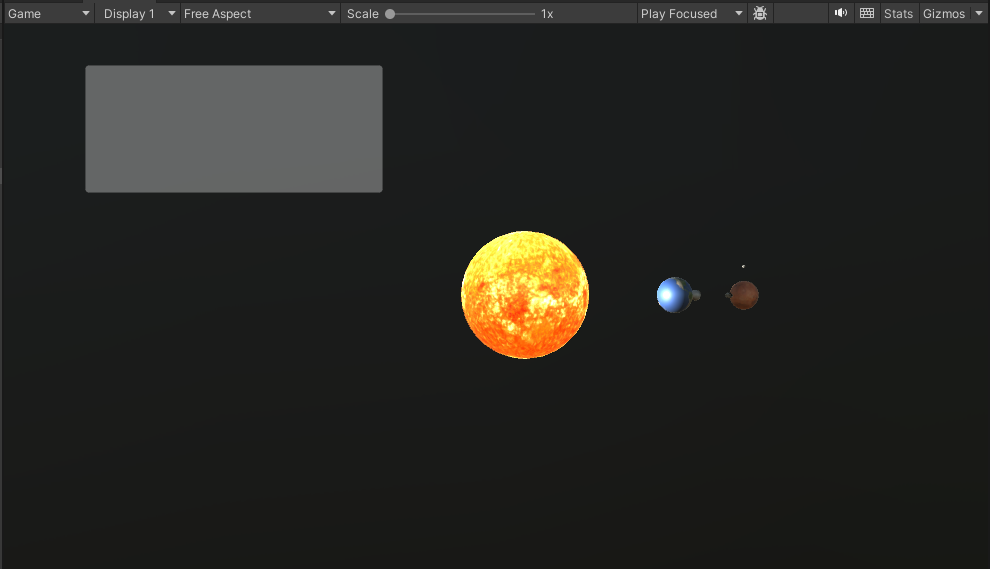
\includegraphics[scale=.50]{fig/panelSoleil-1}
			\caption{Un panel vide actuellement}
			\label{fig:panelSoleil-1}
		\end{center}
%	\end{subfigure}
\end{figure}

\newpage 
\begin{solution}
\subsubsection{Label du Panel}
\begin{itemize}
	\item Ajouter un \texttt{UI > Legacy > Text} nommé "\textit{NomPanelSoleil}" comme enfant de \textit{PanelSoleil}.
	\item \texttt{Inspector > Rect Transform}
	\begin{itemize}
		\item \texttt{Stretch / Stretch > top / left}
			\item \texttt{Pivot X = 0 ; Y = 1}
		\item \texttt{Pos X = 10 ; Pos Y = -10 ; Pos Z = 0}
		\item \texttt{Width = 160 ; Height = 30}
	
	\end{itemize}
	
	\item \texttt{Inspector > Text}
	\begin{itemize}
		\item \texttt{Text >} \textit{Soleil}
		\item \texttt{Character > Font Size >} $24$
	\end{itemize}	
\end{itemize}

\subsubsection{Case à cocher du Panel}
\begin{itemize}
	\item Ajouter un \texttt{UI > Toggle} nommé "\textit{TogglePanelSoleil}" comme enfant de \textit{PanelSoleil}.
	\item \texttt{Inspector > Rect Transform}
	\begin{itemize}
		\item \texttt{Stretch / Stretch > top / left}
		\item \texttt{Pivot X = 0 ; Y = 1}
		\item \texttt{Pos X = 10 ; Pos Y = -50 ; Pos Z = 0}
		\item \texttt{Width = 160 ; Height = 20}	
	\end{itemize}
\end{itemize}

\textit{TogglePanelSoleil} contient lui-même une hiérarchie : 
\begin{itemize}
	\item  \texttt{Background > Checkmark}
	\item \texttt{Label} : à renommer en "\textit{LabelTogglePanelSoleil}" et modifier sa propriété \texttt{Text} pour remplacer "\textit{Toggle}" par "\textit{Animer}".
	\end{itemize}

\subsubsection{Label Vitesse}
\begin{itemize}
	\item Ajouter un \texttt{UI > Legacy > Text} nommé "\textit{VitesseAnimSoleil}" comme enfant de \textit{PanelSoleil}.
	\item \texttt{Inspector > Rect Transform}
	\begin{itemize}
		\item \texttt{Stretch / Stretch > top / left}
		\item \texttt{Pivot X = 0 ; Y = 1}
		\item \texttt{Pos X = 10 ; Pos Y = -80 ; Pos Z = 0}
		\item \texttt{Width = 160 ; Height = 20}	
	\end{itemize}
\end{itemize}

\subsubsection{Slider Vitesse}
\begin{itemize}
	\item Ajouter un \texttt{UI > Slider} nommé "\textit{SliderVitesseAnimSoleil}" comme enfant de \textit{PanelSoleil}.
	\item \texttt{Inspector > Rect Transform}
	\begin{itemize}
		\item \texttt{Stretch / Stretch > top / left}
		\item \texttt{Pivot X = 0 ; Y = 1}
		\item \texttt{Pos X = 10 ; Pos Y = -100 ; Pos Z = 0}
		\item \texttt{Width = 250 ; Height = 20}	
	\end{itemize}
\item \texttt{Inspector > Slider}
\begin{itemize}
	\item \texttt{Min Value = 0}
	\item \texttt{Max Value = 100}
\end{itemize}
\end{itemize}

\subsection{Panel Terre et Panel Mars}
\begin{itemize}
	\item Dupliquer \textit{PanelSoleil} avec \texttt{UI -> Duplicate} dans la \texttt{Hierarchy} en deux exemplaires : \textit{PanelTerre} et \textit{PanelMars}
	\item Vérifier que les propriétés des objets dupliqués sont bien mises à jour (par exemple pour les valeurs \texttt{min} et \texttt{max} des \texttt{Sliders})
	\item Déplacer ces \texttt{Panels} les uns en-dessous (ou à côté) des autres dans le \textit{Canvas} principal
	\item Renommer les objets en conséquence
\end{itemize}

À ce stade, la vue en mode \texttt{Game} devrait ressembler à la fig.~\ref{fig:trois-panels}.
\end{solution}

\newpage 
\begin{figure}[h]
%	\begin{subfigure}{\textwidth}
		\begin{center}
			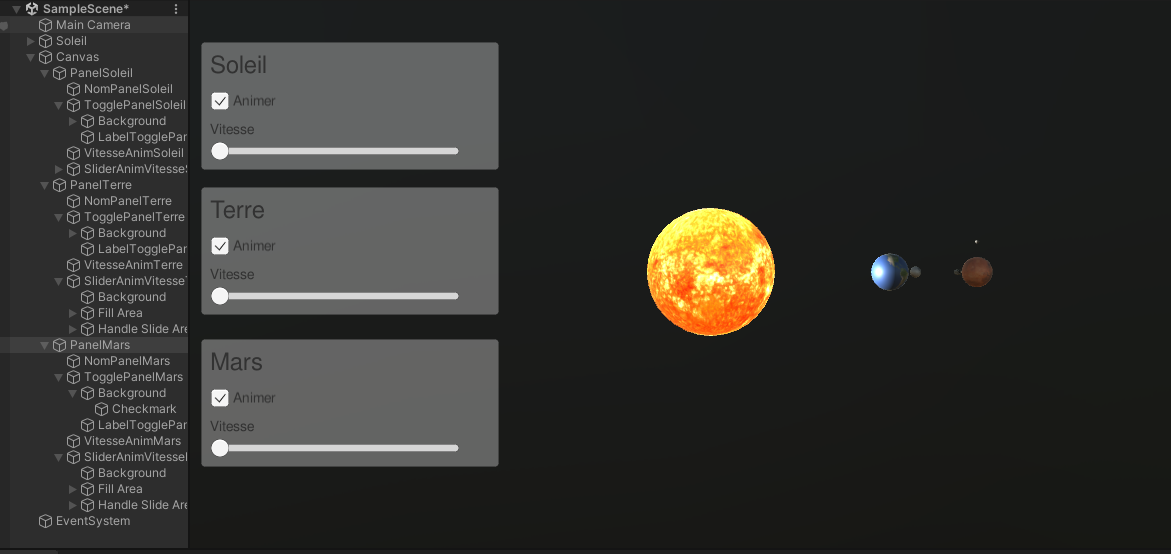
\includegraphics[scale=.50]{fig/trois-panels}
			\caption{Les trois panels}
			\label{fig:trois-panels}
		\end{center}
%	\end{subfigure}
\end{figure}


\fi 


Ensuite sur ce même modèle, réalisez l'interface pour la \textit{Terre} et \textit{Mars} uniquement. Maintenant que vous avez une jolie interface, vous allez réaliser la connexion au écouteur d'événement des boutons d'animation pour contrôler si la rotation de l'astre associé est active ou non. En bref, il vous est demandé de réaliser une fonction, qui détecte les changements de valeur de la \texttt{Checkbox} pour en activer/désactiver l'animation selon la valeur du booléen. 
Pour Le \texttt{Slider}, nous considérons qu'il pourra prendre des valeurs de 0 à 100 et qui contrôlera la vitesse de rotation de l'objet associé.

\ifversionenseignant
\begin{solution}
Dans un premier temps :
\begin{enumerate}
	\item Affecter le même script \lstinline|JeTourne.cs| à la \textit{Terre} et \textit{Mars} avec \texttt{Inspector > Add Component} et la barre de recherche.
	\item Dans le mode \texttt{Game}, désactiver à tour de rôle le \texttt{Toggle} \lstinline|Must Turn| de chaque \lstinline|GameObject| pour mieux observer ses effets.
\end{enumerate}	
	
Ensuite, associer le script suivant nommé \textit{PanelsoleilScript.cs} au \textit{PanelSoleil} avec \texttt{Inspector > Script > New Script}\footnote{Il suffit d'indiquer le nom du script, sans son extension}. Il permet de modifier \textit{via} ce \texttt{Canvas} l'activation/désactivation de la rotation du \textit{Soleil} et sa vitesse. Pour éditer ce script depuis l'\texttt{Inspector}, cliquer sur les 3 points verticaux à droite de ce composant pour faire apparaître un menu contextuel, puis cliquer sur \texttt{Edit}.

\begin{lstlisting}
// Inspire de
// https://docs.unity3d.com/2019.1/Documentation/ScriptReference/UI.Toggle-onValueChanged.html
//Attach this script to a Toggle GameObject. To do this, go to Create>UI>Toggle.
//Set your own Text in the Inspector window
using UnityEngine;
using UnityEngine.UI;
public class PanelSoleilScript : MonoBehaviour
{
	Toggle m_Toggle;
	Slider m_Slider;
	GameObject soleil;
	void Start()
	{
		// m_Toggle est le Toggle enfant de PanelSoleil
		m_Toggle = GetComponentInChildren<Toggle>();
		if (m_Toggle == null)
		Debug.Log("m_Toggle Soleil = nul");
		// m_Slider est le Slider enfant de PanelSoleil
		m_Slider = GetComponentInChildren<Slider>();
		if (m_Slider == null)
		Debug.Log("m_Slider soleil = nul");
		//Add listener for when the state of the Toggle changes, to take action
		m_Toggle.onValueChanged.AddListener(delegate {
			ToggleValueChanged(m_Toggle);
		});
		m_Slider.onValueChanged.AddListener(delegate {
			SliderValueChanged(m_Slider);
		});
		soleil = GameObject.Find("Soleil");
	}
	void ToggleValueChanged(Toggle change)
	{
		soleil.GetComponent<JeTourne>().mustTurn =
		 !soleil.GetComponent<JeTourne>().mustTurn;
	}
	void SliderValueChanged(Slider change)
	{
		soleil.GetComponent<JeTourne>().rotationSpeed = change.value;
	}
}	
\end{lstlisting}

\begin{itemize}
	\item Reprendre le script ci-dessus et modifier les occurrences de \textit{Soleil} par \textit{Terre} ou \textit{Mars}.
	\item Une fois ces scripts compilés, les ajouter respectivement à \textit{PanelTerre} et \textit{PanelMars}.
	\item Ne pas oublier de passer la \texttt{Max Value} de \texttt{SliderVitesseAnimTerre} et SliderVitesseAnimMars à $100$ si nécessaire.
\end{itemize}

\end{solution}
\fi 

\section{Placement de caméra}

Lisez la page du guide suivant: \url{https://docs.unity3d.com/Manual/MultipleCameras.html}. Elle explique les deux façons de contrôler l'affichage d'une caméra simplement.

Pour mettre en pratique les explications du lien, nous vous proposons d'ajouter une caméra locale à la \textit{Lune} (de la \textit{Terre}). Ajoutez des widgets à l'interface pour changer de caméra à la volée comme indiquez dans la documentation.

Pour les explications de la seconde partie, on se propose d'ajouter une 3ème caméra en vue de haut de notre système solaire. Cette vue devra apparaître en miniature dans le bord bas gauche de la fenêtre (ou un autre bord si vous préférez).

\ifversionenseignant
\begin{solution}
\subsection{Ajout d'une Caméra pour la Lune}

\begin{itemize}
	\item Lorsque plusieurs caméras sont utilisées, la caméra visible est celle dont la valeur de la propriété \texttt{depth} est la plus élevée.
	\item Si ce n'est déjà fait, ajouter un \texttt{ GameObject Camera} \textit{Camera Lune} à la \textit{Lune}.
	\item Ajouter un \texttt{Component SkyBox} utilisant "\textit{8k\_stars\_milky\_way}"
	\item Décocher l'\textit{Audio Listener} de cette caméra (il est automatiquement ajouté à chaque nouvelle caméra, mais il ne devrait y en avoir qu'un seul activé à la fois dans la scène).
\end{itemize}	

	
\subsection{Ajout d'un Panel et du script}
\begin{itemize}
	\item Dans le \texttt{Canvas} principal, ajouter un \texttt{Panel} nommé \texttt{PanelCameras} qui comprendra un \texttt{Toggle} nommé \textit{ToggleCameras}, dont le \texttt{Label} contiendra le texte "\textit{Main Camera / Camera Lune}".
	\item Aligner \textit{PanelCameras} avec les autres \texttt{Panels} de \textit{Canvas}.
	\item Associer le script suivant \textit{PermutationCameraScript.cs} à \textit{PanelCameras}.
\end{itemize}	

\begin{lstlisting}
using System.Collections;
using System.Collections.Generic;
using UnityEngine;
using UnityEngine.UI;
// Inspire de https://docs.unity3d.com/Manual/MultipleCameras.html
public class PermutationCamerasScript : MonoBehaviour
{
	// Toggle du Panel associe a ce script
	Toggle m_Toggle;
	// Cameras manipulees
	Camera mainCamera;
	Camera moonCamera;
	// Start is called before the first frame update
	void Start()
	{
		// m_Toggle est le Toggle enfant de PabelCameras
		m_Toggle = GetComponentInChildren<Toggle>();
		if (m_Toggle == null)
		Debug.Log("m_Toggle PanelCameras = nul");
		//Add listener for when the state of the Toggle changes, to take action
		m_Toggle.onValueChanged.AddListener(delegate {
			ToggleValueChanged(m_Toggle);
		});
		mainCamera = getCameraFromParentName("Main Camera");
		mainCamera.enabled = true;
		moonCamera = getCameraFromParentName("Camera Lune");
		moonCamera.enabled = false;
	}
	private Camera getCameraFromParentName(System.String parentName) {
		GameObject cameraObject = GameObject.Find(parentName);
		if (cameraObject == null)
		Debug.Log("CameraObject of " + parentName + "= nul");
		Camera camera = cameraObject.GetComponent<Camera>();
		if (camera == null)
		Debug.Log("Camera of " + parentName + "= nul");
		return camera;
	}
	void ToggleValueChanged(Toggle change)
	{
		mainCamera.enabled = !mainCamera.enabled;
		moonCamera.enabled = !moonCamera.enabled;
	}
}	
\end{lstlisting}
	
	\subsection{3ème caméra}
\begin{itemize}
	\item Dans la \texttt{Hierarchy}, ajouter une \texttt{Camera} et la nommer "\textit{Camera Up View}".
	\item La placer et l'orienter de manière à offrir une "vue de dessus" du système solaire, par exemple, dans l'\texttt{Inspector}:
	\begin{itemize}
		\item \texttt{Transform > Position -> X = 0 ; Y = 15 ; Z = -0.8}
		\item \texttt{Transform > Rotation -> X = 84.43 ; Y = -20.639 ; Z = -124.044}
		\item \texttt{Camera > Field of View = 28}
		\item \texttt{Depth = 2}: valeur supérieure à la propriété de même nom des autres caméras 
		\item \texttt{ViewPort Rect > X = 0.8 ; Y = 0}: place le rectangle de cette vue en bas à droite de la scène finale
		\item \texttt{ViewPort Rect > W = 0.2 ; H = 0.2}: facteurs d'échelle des dimensions du rectangle de vue
	\end{itemize}
	\item Ajouter un \texttt{Component SkyBox} utilisant "\textit{8k\_stars\_milky\_way}".
	\item Décocher l'\textit{Audio Listener} de cette caméra.
\end{itemize}	
\end{solution}

À ce stade, l'interface ressemble à celle de la fig.~\ref{fig:camera-haut} (la vue de \texttt{Camera Up View} est affichée en bas à droite de l'écran)
\begin{figure}[h]
		\begin{center}
			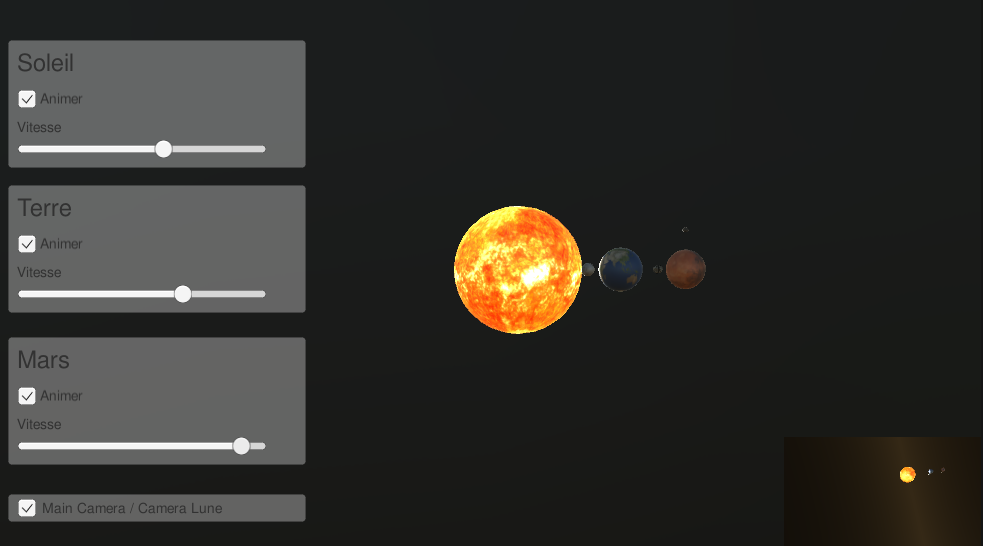
\includegraphics[scale=.50]{fig/camera-haut}
			\caption{Interface avec \texttt{Camera Up View}}
			\label{fig:camera-haut}
		\end{center}
\end{figure}

\fi 
	

\section{Pour aller plus loin}

La mécanique céleste mise en place jusqu'à présent est vraiment catastrophique, mais offre un cadre suffisant pour l'apprentissage des mécaniques. Nous vous proposons d'ajouter une comète cyclique (ou autre astre) qui n'est plus sous-fils du Soleil, mais bien un objet quelconques.

Pour pouvoir animer votre comète vous allez devoir lui fournir une équation qui va traduire sa trajectoire pour cela je vous propose de vous inspirez du lien suivant \url{https://fr.wikipedia.org/wiki/Trajectoire_d%27une_com%C3%A8te}
ou d'utiliser l'équation d'un cercle autour du soleil par exemple.

\ifversionenseignant
\begin{solution}
L'objectif est de créer un objet qui tourne autour du \textit{Soleil} mais n'appartient pas à sa hiérarchie.

\begin{itemize}
	\item Importer un objet 3D au format \texttt{.obj} pour représenter un nouvel astéroïde, par exemple \href{https://nasa3d.arc.nasa.gov/detail/bennu}{Bennu}\footnote{Ce maillage n'a pas de normale incluses, mais \texttt{Unity} les recalcule automatiquement.}.
	\item Placer cet objet dans le \texttt{Project > Assets > Images}.
	\item Déplacer cet objet depuis \texttt{Project} vers \texttt{Hierarchy}, ce qui l'ajoute à la scène. Sa position initiale est en \textit{(X=0, Y=0, Z=0)} : le déplacer sur un autre axe, par exemple en \textit{(X=2.2, Y=1.5, Z=0)}.
	\item Cet objet contient un enfant nommé "\textit{default}" : associer à ce dernier un enfant de type \texttt{Trail} : \texttt{bouton droit > Effects > Trail.} 
	\item Modifier la Position de ce \texttt{Trail} en \textit{()X = 0 ; Y = 0 ; Z = 0)} pour le "coller" sur \textit{default}.
	\item Modifier le \texttt{Trail Renderer} de ce \texttt{Trail}:
	\begin{itemize}
		\item en diminuant sa largeur \texttt{Width} (valeur \textit{0.2} par exemple);
		\item en modifiant éventuellement sa propriété \texttt{Color};
		\item en modifiant la propriété \texttt{Time} correspondant à la durée de vie de la trace laissée par l'objet.
	\end{itemize}
\end{itemize}

Le script suivant \texttt{TrajectoiresScript.cs} associé à \textit{Bennu} permet de créer une trajectoire elliptique autour du centre du repère global, avec le soleil constituant l'un des foyers de l'ellipse. Les attributs \texttt{Semi Major} et \texttt{Ecliptic Angle} de \texttt{Bennu} accessibles depuis l'\texttt{Inspector} permettent de changer la forme de l'ellipse (un cercle pour \texttt{Ecliptic Angle} = $0$, une ellipse de plus en plus allongée lorsque \texttt{Ecliptic Angle} tend vers \texttt{Semi Major}).

\begin{lstlisting}
using System.Collections;
using System.Collections.Generic;
using UnityEngine;
using UnityEngine.UIElements;

// Trajectoire circulaire ou elliptique en utilisant le soleil comme foyer d'une ellipse

public class TrajectoiresScript : MonoBehaviour
{
	private GameObject soleil;
	
	public float semiMajor = 1f ; // demi-grand axe de l'ellipse > 0
	
	// angle de rotation entre ce GameObject et le soleil ; 
	// a calculer a chaque pas de temps 
	public float angle = 0f; // a convertir en radians
	
	// inclinaison de l'ellipse (en degres) en restant dans le meme plan de
	// l'ecliptique
	public float eclipticAngle = 0f; // a convertir en radians
	
	// L'excentricite est definie selon la distance entre le centre de l'ellipse, 
	// l'un de ses foyers et le demi-grand axe
	private float eccentricity;
	
	// Start is called before the first frame update
	void Start()
	{
		soleil = GameObject.Find("Soleil");
		if (soleil == null) {
			Debug.Log("TrajectoiresScript: soleil = null");
		}
	}
	// Update is called once per frame
	void Update()
	{
	}
	// FixedUpdate is called at fixed frames. To use with rigid Bodies
	// https://docs.unity3d.com/ScriptReference/MonoBehaviour.FixedUpdate.html
	void FixedUpdate()
	{
		// En toute generalite, l'excentricite est definie sur un axe, 
		// X par convention.
		// Formule generale : 
		// excentricite = Abs(centre de l'ellipse.X - foyer de l'ellipse.X) /
		//   demi-grand axe
		// => et cette valeur doit etre comprise dans [0 ; 1[
		
		// On suppose ici que le centre de l'ellipse est le centre du 
		//  repere global (0,0,0)
		eccentricity = Mathf.Abs(soleil.transform.position.x) / semiMajor;
		Debug.Log("eccentricity = " + eccentricity);
		
		// semiMinor = demi-petit axe de l'ellipse
		//=> semiMajor et semiMinor sont lies a l'excentricite de l'ellipse E 
		//  par semiMinor = semiMajor * sqrt(1 - E*E)
		
		// => si semiMajor et semiMinor sont egales, l'orbite est un cercle 
		//  (facile a voir avec tiltEclipticAngle = 0)
		float semiMinor = semiMajor *Mathf.Sqrt(1 - eccentricity * eccentricity);
		float angleRad = Mathf.Deg2Rad * angle;
		float angleRadCos = Mathf.Cos(angleRad);
		float angleRadSin = Mathf.Sin(angleRad);
		float eclipticAngleRad = Mathf.Deg2Rad * eclipticAngle;
		float eclipticAngleRadCos = Mathf.Cos(eclipticAngleRad);
		float eclipticAngleRadSin = Mathf.Sin(eclipticAngleRad);
		
		// Remarque: Multiplier par Time.fixedDeltaTime (=0.02) donne des 
		//  resultats proches de 0
		// les coordonnees X et Z resultantes sont donc proches de 0 => 
		//  ce GameObjet ne se deplace donc quasiment pas
		// => on "equilibre" les coordonnees en multipliant par 10
		this.gameObject.transform.position = 
		  new Vector3(((semiMajor * angleRadCos * eclipticAngleRadCos) - 
		  (semiMajor * angleRadSin * eclipticAngleRadSin)) * 
		  Time.fixedDeltaTime * 10f,
		
		  0,
		  
		  ((semiMinor * angleRadCos * eclipticAngleRadSin) - 
		  (semiMinor * angleRadSin * eclipticAngleRadCos)) * 
		  Time.fixedDeltaTime * 10f);
		  
		  angle += 1f;//can be used as speed
		  
		  if (angle > 360f) {
			angle = 0f;
		}
		
		Debug.Log("new X = " + this.gameObject.transform.position.x + 
		  ", new Z = " + this.gameObject.transform.position.z);
		
		Debug.Log("soleil.X = " + soleil.transform.position.x); 
		// On peut faire varier la position du Soleil en X, 
		//  sans depasser la valeur de semiMajor
		
		Debug.Log("Time.fixedDeltaTime = " + Time.fixedDeltaTime);
	}
}
	
\end{lstlisting}

La fig.~\ref{fig:bennu-ellipse} affiche la trace laissée par \texttt{Bennu} en cours d'animation.
\end{solution}
\begin{figure}[!h]
	\begin{center}
		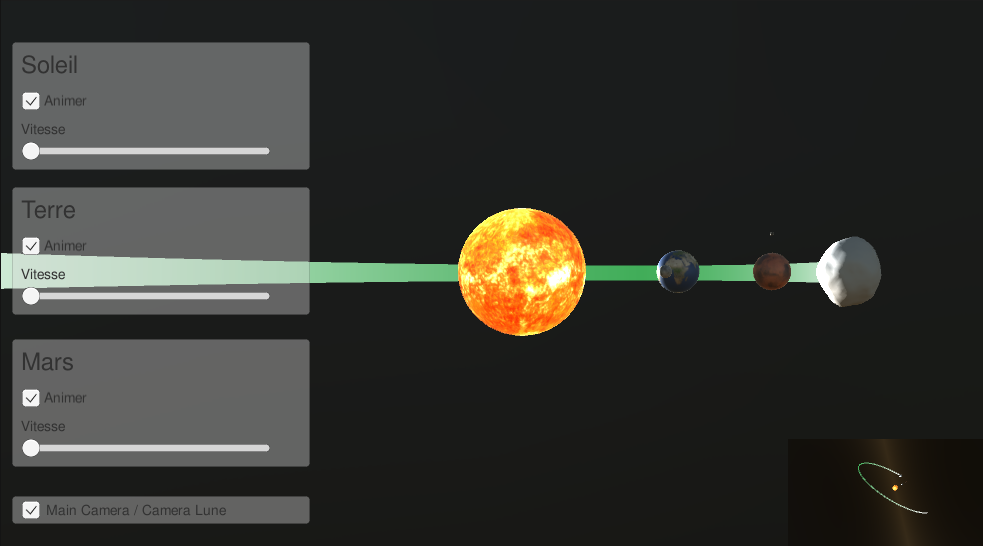
\includegraphics[scale=.50]{fig/bennu-ellipse}
		\caption{Interface avec \texttt{Bennu} en mouvement}
		\label{fig:bennu-ellipse}
	\end{center}
\end{figure}
\fi 

\newpage 

\section{Toujours plus loin}

Si vous avez tout fini, nous pouvons complexifier les traitements en regardant la documentation:
\begin{itemize}
	\item En utilisant la fonction \texttt{LookAt} dans la classe \texttt{Transform}, ajoutez pour chaque interface un bouton \texttt{'Center View'} qui centre la vue de la caméra principale vers l'astre associé.
	\item Modifier votre traitement précédent pour que la caméra tourne doucement vers sa position finale pour éviter de perdre l'utilisateur ou lui donner des nausées. Pour cela, nous utiliserons une interpolation linéaire ou sphérique  entre le point de vue de départ et le point de vue d'arrivée avec une vitesse constante.
\end{itemize}

\ifversionenseignant
\begin{solution}

\subsection{Création des Toggles}

L'objectif est de pouvoir sélectionner la planète sur laquelle la vue de la caméra principale sera centrée, ou bien de revenir à l'orientation originale de la caméra.

\begin{itemize}
	\item Repositionner les \texttt{Panels} du \texttt{Canvas} principal pour ajouter un nouveau \texttt{Panel} nommé "\textit{PanelLookAt}".
	\item Ajouter dans  \textit{PanelLookAt} un \texttt{Label} nommé \textit{NomPanelLookAt} et contenant le \texttt{Text} "\textit{Cameras LookAt}".
	\item Ajouter une succession de \texttt{Toggles} nommés respectivement \textit{ToggleSoleil}, \textit{ToggleTerre}, \textit{ToggleMars} et \textit{ToggleOriginal} avec les \texttt{Text} de leurs \texttt{Labels} respectifs : \textit{Soleil}, \textit{Terre}, \textit{Mars} et \textit{Original}.
	\item Pour chaque \texttt{Toggle} :
	\begin{itemize}
		\item 	Désactiver la propriété \texttt{IsOn}, sauf pour \textit{Original}
		\item  Ajouter le \texttt{Component} \texttt{Layout Element} et spécifier la propriété \texttt{LayoutElement -> Preferred Height} = $20$ (coche activée).		
	\end{itemize}	
\end{itemize}

\subsection{ToggleGroup}

On va maintenant regrouper tous ces \texttt{Toggle} dans un \texttt{ToggleGroup}.
\begin{itemize}
	\item Dans \textit{PanelLookAt}, créer un \texttt{Create Empty} nommé \textit{ToggleGroupLookAt}. Il s'agit d'un \texttt{GameObject} quasiment vide avec des propriétés minimales, que l'on va utiliser comme un conteneur. Le redimensionner au besoin pour qu'il tienne dans  \textit{PanelLookAt}.
	\item Modifier la hiérarchie pour que \textit{ToggleGroupLookAt} devienne le parent des \texttt{Toggles}.
	\item Ajouter à \textit{ToggleGroupLookAt} le \texttt{Component Toggle Group} et désactiver le booléen \texttt{Allow Switch Off} de ce dernier pour faire en sorte qu'un seul \texttt{Toggle} enfant soit sélectionné à la fois.
	\item Ajouter le \texttt{Component Vertical Layout Group} à \textit{ToggleGroupLookAt} si les \texttt{Toggles} sont disposés verticalement ; le \texttt{Component Horizontal Layout Group} sinon.
	\item Dans ce \texttt{Component}, désactiver la propriété \texttt{Child Force Expand > Height} pour \texttt{Vertical Layout Group} ou \texttt{Child Force Expand > Width} pour \texttt{Horizontal Layout Group}.
	\item Ajouter le script suivant \textit{ToggleGroupLookAtScript.cs} à \textit{ToggleGroupLookAt}. Il permet de récupérer la planète associée au \texttt{Toggle} sélectionné.
\end{itemize}

\begin{lstlisting}
using UnityEngine;
using System.Collections;
using UnityEngine.UI;
using System.Linq;
public class ToggleGroupLookAtScript : MonoBehaviour {
  ToggleGroup m_ToggleGroup;
  Toggle m_PreviousToggle;
  Toggle m_SelectedToggle;
	
  public Toggle GetCurrentSelection() {
  	return m_ToggleGroup.ActiveToggles().FirstOrDefault();
  }
	
  public Toggle GetPreviousSelection() {
	return m_PreviousToggle;
  }
	
  void Start() {
	m_ToggleGroup = GetComponent<ToggleGroup>();
	m_PreviousToggle = GetCurrentSelection();
	m_SelectedToggle = GetCurrentSelection();
	Debug.Log("[ToggleGroupLookAtScript][Start] m_PreviousToggle = " +
	m_PreviousToggle.name + ", m_SelectedToggle = " +
	m_SelectedToggle.name);
  }
	
  public GameObject GetGameObjectFromToggle(Toggle toggle) {
	switch(toggle.name) {
		case "ToggleSoleil":
			return GameObject.Find("Soleil");
		case "ToggleTerre":
			return GameObject.Find("Terre");
		case "ToggleMars":
			return GameObject.Find("Mars");
		case "ToggleOriginal":
			return GameObject.Find("Main Camera");
		default:
			return null;
	}
  }

  void Update() {
	if (GetCurrentSelection() != m_SelectedToggle) {
		m_PreviousToggle = m_SelectedToggle;
		m_SelectedToggle = GetCurrentSelection();

		Debug.Log("[ToggleGroupLookAtScript][Update] m_PreviousToggle = " +

		m_PreviousToggle.name + ", m_SelectedToggle = " +
		m_SelectedToggle.name);
	}
  }
}
\end{lstlisting}

Sélectionner l'ensemble des \texttt{Toggle} enfants, puis cliquer sur \texttt{ToggleGroupLookAt} et le déplacer à la souris dans la propriété \texttt{Toggle > Group} des enfants sélectionnés. La valeur de cette propriété passe de \texttt{None (Toggle Group)} à \texttt{ToggleGroupLookAt (Toggle Group)}.\\

On peut tester l'activation des boutons en démarrant la scène et en cliquant sur chaque bouton du groupe, ce qui désactive le bouton précédent.

\subsection{Changement de caméra}

Le script \textit{LookAtPlanetSlerpScript.cs} ci-dessous est attaché à chaque \texttt{Toggle} enfant de \texttt{ToggleGroupLookAt}. Pour chacun d'eux, il vérifie s'il est sélectionné et dans ce cas,  si le \texttt{Toggle} précédemment sélectionné est différent, change la position de la caméra d'une planète à l'autre, selon une interpolation sphérique basée sur les quaternions.

\begin{lstlisting}
// Script attache aux GameObject "Toggle" enfants de ToggleGroupLookAt pour
//  centrer la vue de la camera principale sur une planete donnee, 
// ou revenir a l'orientation originale.

// Attention : chaque Toggle possede sa propre instance de ce script.
// Donc toutes les variables du script sont definies independamment pour chaque Toggle
// (elles ne sont pas partagees)

// Inspire de
// https://docs.unity3d.com/2019.1/Documentation/ScriptReference/UI.Toggle-onValueChanged.html
// Set your own Text in the Inspector window

using UnityEngine;
using UnityEngine.UI;
using System.Collections;
using System.Linq;
public class LookAtPlanetScriptSlerp : MonoBehaviour
{
  Toggle m_Toggle;
	
  GameObject m_MainCamera;
	
  float m_TimeCount = 0.0f;
	
  bool m_EnableInterpolation = false;
	
  ToggleGroup m_ToggleGroup;
	
  Quaternion m_MainCameraInitialRotation;
	
  public ToggleGroupLookAtScript m_ToggleGroupLookAtScript;
	
  void Start() {
    Debug.Log("[LookAtPlanetSlerpScript] [1]");

    // On recupere le script identifiant la planete vers laquelle deplacer la camera
    m_ToggleGroupLookAtScript =
      GameObject.FindObjectOfType(typeof(ToggleGroupLookAtScript))
    	as ToggleGroupLookAtScript;
		
    Debug.Log("[LookAtPlanetSlerpScript] [2]");
				
    // ToggleGroup parent
    m_ToggleGroup = GetComponentInParent<ToggleGroup>();
    if (m_ToggleGroup == null) {
    	Debug.Log("[LookAtPlanetSlerpScript] m_ToggleGroup = nul");
    }
    else {
      Debug.Log("[LookAtPlanetSlerpScript] m_ToggleGroup = " + m_ToggleGroup.name);
    }
		
    // m_Toggle est le Toggle "enfant" de ce GameObject (en fait le Toggle actuel)
    m_Toggle = GetComponentInChildren<Toggle>();

    if (m_Toggle == null)
       Debug.Log("[LookAtPlanetSlerpScript] m_Toggle = nul");
		
    // Add listener for when the state of the Toggle changes, to take action
    m_Toggle.onValueChanged.AddListener(delegate {
      ToggleValueChanged(m_Toggle);
    });
		
    // On recherche la [Main Camera] pour la position originale
    m_MainCamera = GameObject.Find("Main Camera");
		
    // Enregistrement de la rotation de la camera originale
    m_MainCameraInitialRotation = m_MainCamera.transform.rotation;
    if (m_MainCamera == null) {
    	Debug.Log("[LookAtPlanetSlerpScript] m_MainCamera = nul");
    }
  }
	
  void ToggleValueChanged(Toggle change) {
    if (m_Toggle.isOn) {
		Debug.Log("[LookAtPlanetSlerpScript] m_Toggle = " + m_Toggle.isOn + 
		  " pour " + name);
    	m_EnableInterpolation = true;
	}
  }
	
  void FixedUpdate() {
    Toggle selectedToggle = m_ToggleGroupLookAtScript.GetCurrentSelection();
    Toggle previousToggle = m_ToggleGroupLookAtScript.GetPreviousSelection();
		
    if (m_Toggle.isOn) { // Ce Toggle est active
			
    // Recuperation de la planete associee
    GameObject selectedObject =
      m_ToggleGroupLookAtScript.GetGameObjectFromToggle(selectedToggle);
			
    if (m_EnableInterpolation) {
      if (selectedToggle != previousToggle) {
        if (selectedObject != m_MainCamera) {
          GameObject previousObject = 
            m_ToggleGroupLookAtScript.GetGameObjectFromToggle(previousToggle);
						
          if (selectedObject == null || previousObject == null) {
            Debug.Log("[LookAtPlanetSlerpScript][Update] selectedObject = nul ou " +
             "previousObject = nul");
          }
						
// https://docs.unity3d.com/2022.2/Documentation/ScriptReference/Quaternion.LookRotation.html
          Vector3 relativePos = selectedObject.transform.position - 
            m_MainCamera.transform.position;
						
          Quaternion rotation = Quaternion.LookRotation(relativePos, Vector3.up);
						
// https://docs.unity3d.com/2022.2/Documentation/ScriptReference/Quaternion.Slerp.html
// [m_timeCount] varie entre 0 (axe de rotation initial) et 1 (axe de rotation final)
// Sa valeur est mise a jour a chaque frame.
          m_MainCamera.transform.rotation =
          Quaternion.Slerp(m_MainCamera.transform.rotation,
                           rotation,
                           m_TimeCount);											
        }
					
        else { // selectedObject == m_MainCamera
          GameObject previousObject = 
            m_ToggleGroupLookAtScript.GetGameObjectFromToggle(previousToggle);
						
          if (selectedObject == null || previousObject == null) {
            Debug.Log("[LookAtPlanetSlerpScript][Update] selectedObject = nul ou " +
              "previousObject = nul");
          }
          m_MainCamera.transform.rotation = 
            Quaternion.Slerp(m_MainCamera.transform.rotation,
                             m_MainCameraInitialRotation,
                             m_TimeCount);
        }
        UpdateTimeCount();
      }
    }
    else if (m_MainCamera != selectedObject) {
      m_MainCamera.transform.LookAt(selectedObject.transform);
    }
   }
 }
	
  void UpdateTimeCount() {
    Debug.Log("[LookAtPlanetSlerpScript][Update] rotation = " + 
      m_MainCamera.transform.rotation);
    m_TimeCount += Time.deltaTime;
		
    // [m_TimeCount] doit rester dans l'intervalle  [0; 1].
    if (m_TimeCount > 1.0f) {
      m_TimeCount = 0.0f;
			
    // On est arrive sur l'axe de rotation final : l'interpolation stoppe
      m_EnableInterpolation = false;
    }
  }
}
	
\end{lstlisting}

La fig.~\ref{fig:cam-mars} illustre l'animation avec la caméra centrée sur \textit{Mars}.

\end{solution}
\begin{figure}[!h]
	\begin{center}
		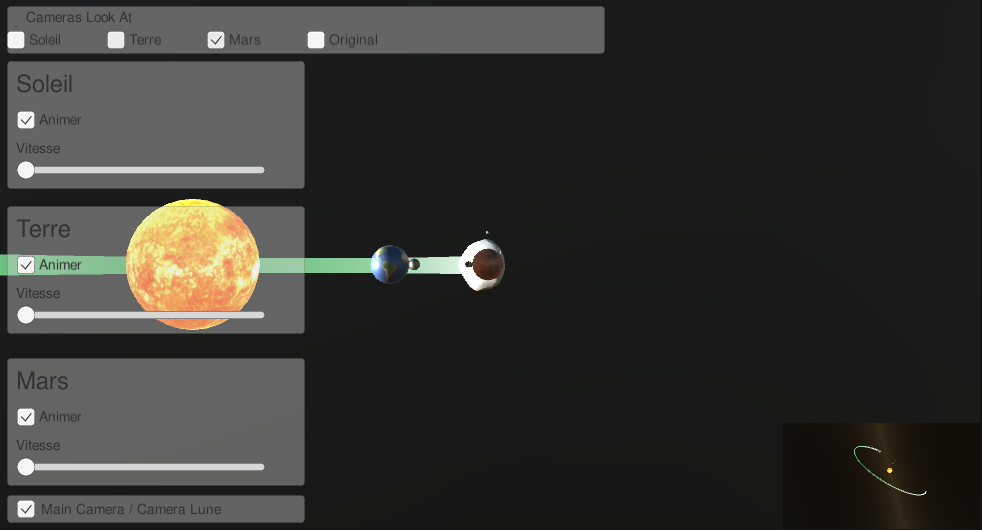
\includegraphics[scale=.50]{fig/camera-centree-Mars}
		\caption{Caméra centrée sur Mars}
		\label{fig:cam-mars}
	\end{center}
\end{figure}

\fi 

\end{document}
